\documentclass[12pt]{article}

\usepackage{sbc-template}
\usepackage{makeidx,graphicx}
\usepackage[utf8]{inputenc}
\usepackage[brazil]{babel}
\usepackage[T1]{fontenc}
\usepackage{listings}
\usepackage{xcolor}
\usepackage{float} 

\lstset{
    language=Python,
    basicstyle=\ttfamily\small,
    keywordstyle=\color{blue},
    stringstyle=\color{red},
    commentstyle=\color{green!50!black},
    breaklines=true,
    showstringspaces=false,
    numbers=left,
    numberstyle=\tiny\color{gray},
    frame=single
}

\title{Relatório Técnico: Implementação de Montador Simplificado RISC-V}

\author{Tadeu Miller, Arthur Felipe}

\address{Departamento de Ciência da Computação -- Universidade Federal de Viçosa (UFV)\\
  Campus Florestal -- MG -- Brasil
  \email{tadeu.andrade@ufv.br; arthur.f.campos@ufv.br} 
}

\begin{document} 

\maketitle

\begin{abstract}
  This report describes the development of a simplified RISC-V assembler 
  in Python. The software converts assembly instructions into 32-bit machine 
  code, supporting R, I, S, and B instruction formats, pseudo-instructions, 
  and multiple numeric bases.
\end{abstract}

\begin{resumo}
  Este relatório descreve o desenvolvimento de um montador RISC-V 
  simplificado em Python. O software converte instruções assembly em código 
  de máquina de 32 bits, suportando os formatos de instrução R, I, S e B, 
  pseudo-instruções e múltiplas bases numéricas.
\end{resumo}

\section{Introdução}
O objetivo deste trabalho prático é a implementação de um montador capaz de traduzir um conjunto de instruções da arquitetura RISC-V. Compreender o processo de montagem, bem como o software interage com o hardware é fundamental para compreender os computadores atuais \cite{patterson_hennessy}. O programa desenvolvido lê arquivos de texto contendo código fonte em assembly (extensão \texttt{.asm}) e gera as representações binárias, garantindo a compatibilidade com simuladores.

\section{Instalações e Requisitos}
O programa foi desenvolvido em \textbf{Python}. A escolha da linguagem se deu pela facilidade na manipulação das strings e dos dicionários. Para rodar o projeto em um ambiente Linux, siga os passos:

\begin{enumerate}
    \item Verifique se o interpretador Python 3 está instalado na máquina:
    \begin{lstlisting}[language=bash]
    sudo apt update
    sudo apt install python3
    \end{lstlisting}
    \item A execução não exige a instalação de outras bibliotecas externas via \texttt{pip}, pois o código utiliza apenas a biblioteca nativa \texttt{sys}.
\end{enumerate}

\section{Guia de Execução}
O script identifica como o usuário deseja receber a saída com base nos argumentos passados via terminal, através da função \texttt{main}:

\subsection{Saída no próprio Terminal}
\begin{lstlisting}[language=bash]
python3 montador.py entrada.asm
\end{lstlisting}

\subsection{Escrita em Arquivo}
Para salvar o resultado em um arquivo, utilizamos o parâmetro \texttt{-o}. O código valida a presença do argumento para evitar erros de execução:
\begin{lstlisting}[language=bash]
python3 montador.py entrada.asm -o saida.txt
\end{lstlisting}

\section{Detalhamento da Implementação}
A implementação seguiu o manual de instruções da arquitetura RISC-V \cite{riscv_isa} e foi dividida nos módulos descritos a seguir.

\subsection{Tratamento de strings}
Utilizamos a função \texttt{replace} para remover vírgulas e parênteses, permitindo que o \texttt{split()} isole tudo em uma lista. A função \texttt{registrador\_para\_binario(reg)} é responsável por converter os nomes dos registradores (Exemplo: x3) em endereços binários de 5 bits.

\subsection{Imediatos e várias bases}
O suporte a múltiplas bases (decimal, hex e binário) é feito via \texttt{int(valor, 0)} \cite{python_bitwise}. Para imediatos negativos, aplicamos um \texttt{AND} bit a bit para gerar o complemento de 2 correto em 12 ou 13 bits.

\begin{lstlisting}[language=Python]
def imediato_para_binario(imediato, bits=12):
    numero = int(imediato, 0)
    binario = format(numero & ((1 << bits)-1), f'0{bits}b')
    return binario
\end{lstlisting}

\subsection{Tipo de instrução S}
O formato S (instruções de store) divide o imediato de 12 bits em dois campos
não contíguos na instrução final: os 7 bits superiores ocupam os bits 31--25,
e os 5 bits inferiores ocupam os bits 11--7.

\begin{lstlisting}[language=Python]
imm_1 = imm_bin[0:7]   # bits 11 a 5 -> posicao 31-25
imm_2 = imm_bin[7:12]  # bits 4 a 0  -> posicao 11-7

binario_final = f'{imm_1}{rs2}{rs1}{funct3}{imm_2}{opcode}'
\end{lstlisting}

\subsection{Tipo de instrução B}
O formato B (instruções de branch, também conhecidas como os if/else de linguagens de alto nível) exige um certo "embaralhamento" dos bits dentro da instrução final. Resolvemos isso fatiando a string gerada pela função de imediato, acessando os caracteres pelos índices e juntando-os na ordem certa.

\begin{lstlisting}[language=Python]
# Exemplo de reorganizacao dos bits para o Tipo B
imm_1 = imm_bin[0]    # bit 12
imm_2 = imm_bin[2:8]  # bits 10 a 5
imm_3 = imm_bin[8:12] # bits 4 a 1
imm_4 = imm_bin[1]    # bit 11
        
binario_final = f'{imm_1}{imm_2}{rs2}{rs1}{funct3}{imm_3}{imm_4}{opcode}'
\end{lstlisting}

\subsection{Pseudo-instruções}
O montador tem suporte a pseudo-instruções para simplificar a programação:
\begin{itemize}
    \item \texttt{mv rd, rs} $\rightarrow$ \texttt{add rd, rs, x0}.
    \item \texttt{li rd, imm} $\rightarrow$ \texttt{ori rd, x0, imm}.
    \item \texttt{bnez rs, offset} $\rightarrow$ \texttt{bne rs, x0, offset}.
\end{itemize}

\subsection{Fluxo de Controle e Tratamento de Erros}
A função \texttt{main} coordena a leitura e escrita de arquivos. Caso uma instrução resulte num binário inválido ou não seja reconhecida, o programa utiliza \texttt{sys.exit(1)}. Isso evita que os binários finais gerados (ou o arquivo final gerado) contenha lixo. Assim garantimos que o montador gera código funcional para um simulador RISC-V.

\section{Resultados e validação}
A validação consistiu em comparar as saídas geradas pelo montador com os padrões dos binários definidos para a arquitetura RISC-V, garantindo que cada campo (opcode, funct, registradores) estivesse na posição certa.

\subsection{Testes por Formato}
As Figuras abaixo demonstram a correta alocação dos campos e o fatiamento de bits para os formatos R, I, S e B.

\begin{figure}[H]
\centering
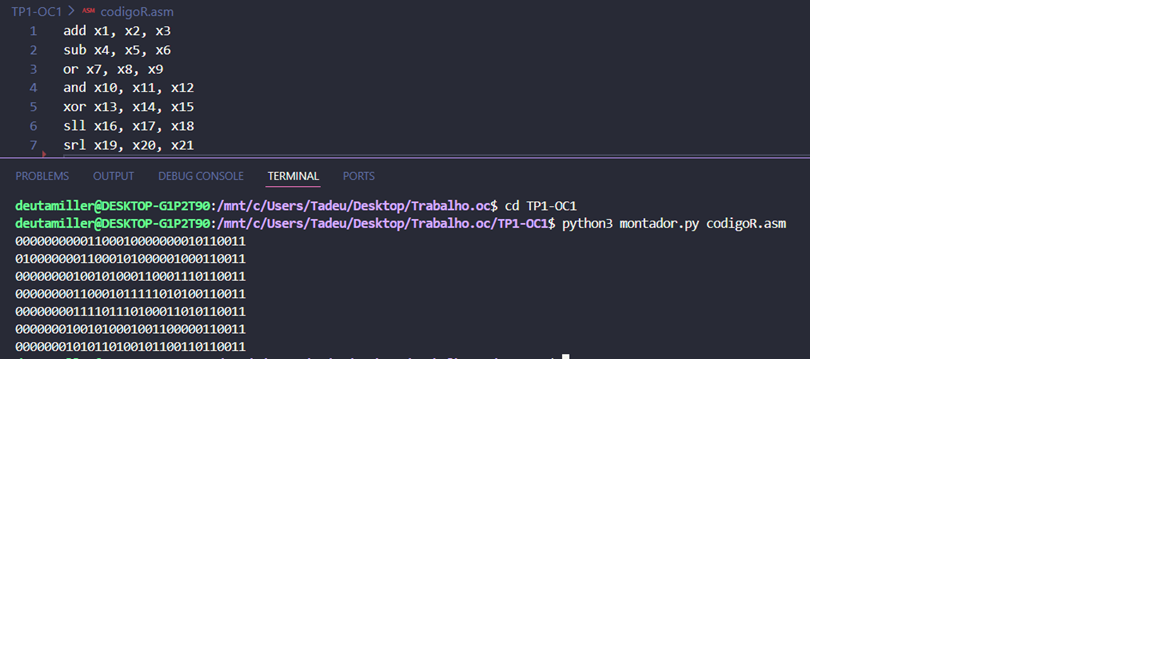
\includegraphics[width=0.8\textwidth]{CodigoR.png}
\caption{Saída binária no terminal para instruções do tipo R.}
\label{fig:tipoR}
\end{figure}

\begin{figure}[H]
\centering
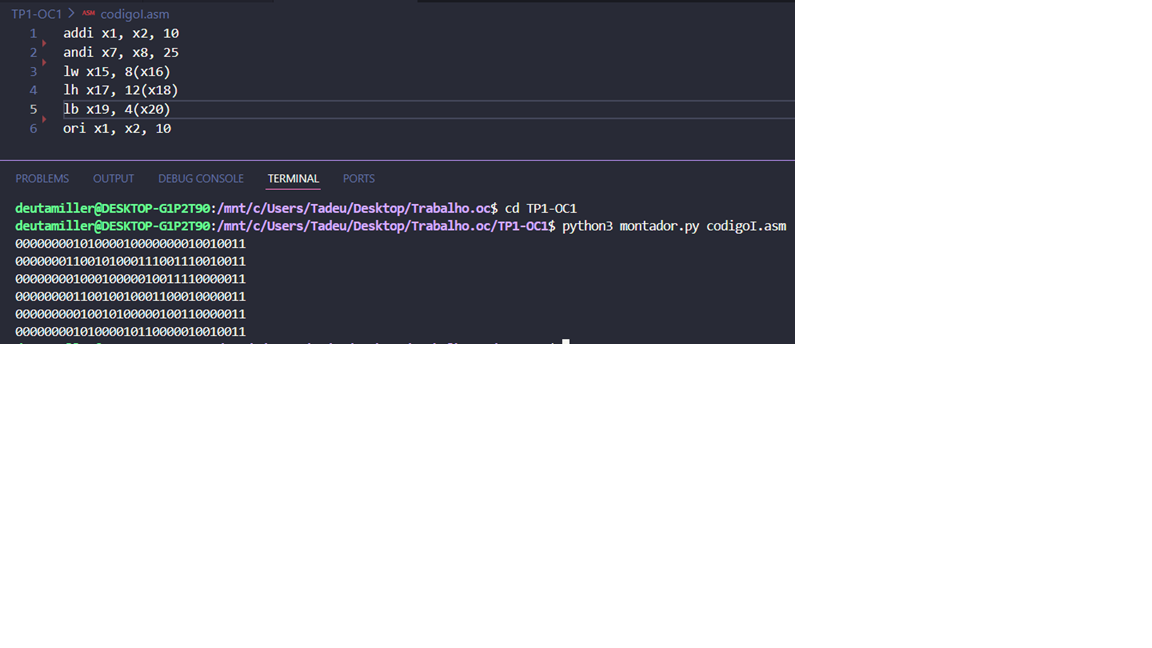
\includegraphics[width=0.8\textwidth]{codigoI.png}
\caption{Processamento de instruções do tipo I.}
\label{fig:tipoI}
\end{figure}

\begin{figure}[H]
\centering
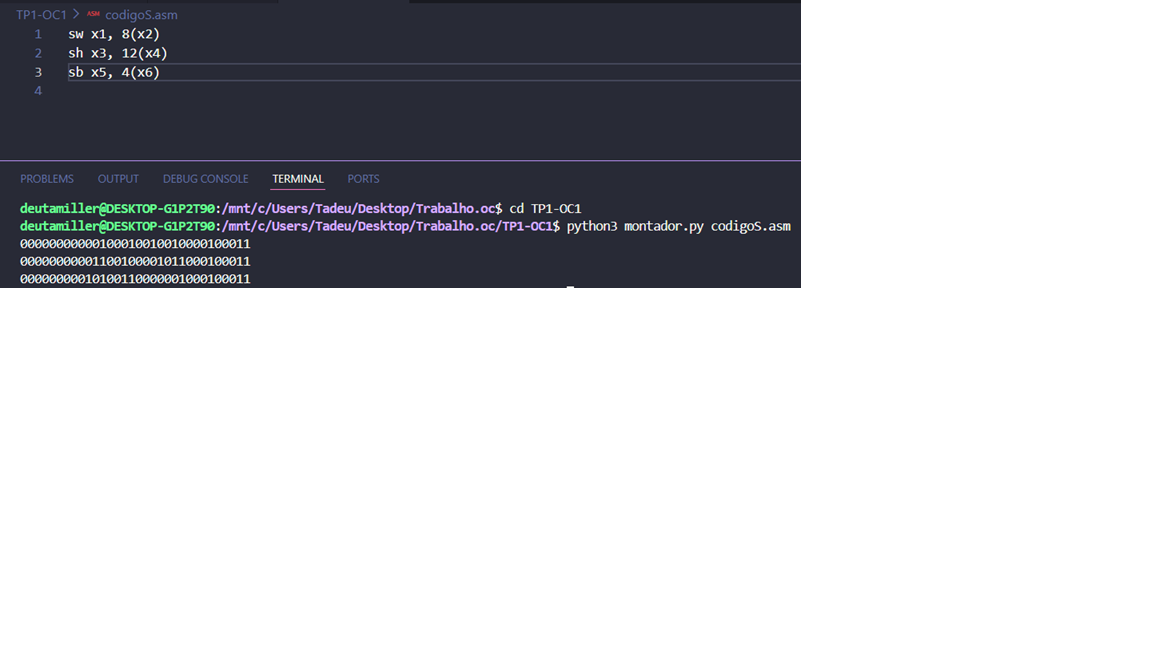
\includegraphics[width=0.8\textwidth]{codigoS.png}
\caption{Montagem de instruções Tipo S.}
\label{fig:tipoS}
\end{figure}

\begin{figure}[H]
\centering
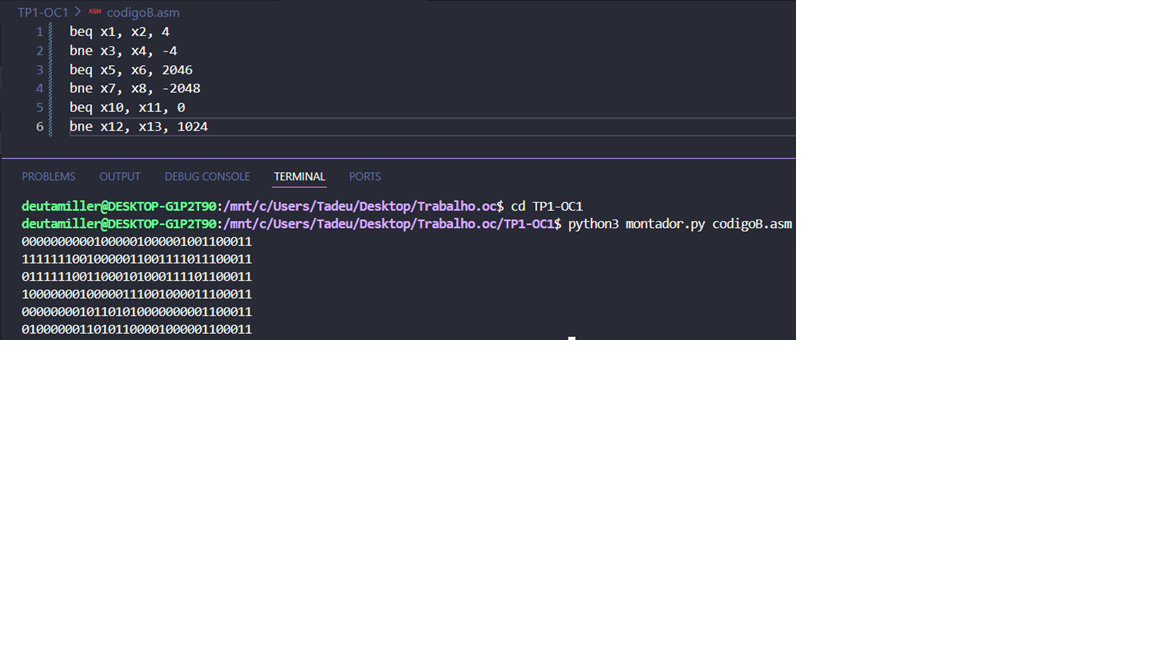
\includegraphics[width=0.8\textwidth]{codigoB.png}
\caption{Montagem de instruções Tipo B.}
\label{fig:tipoB}
\end{figure}

\subsection{Teste Geral}
A Figura \ref{fig:teste_geral} demonstra a conversão de um arquivo com instruções mistas, validando a lógica do montador.

\begin{figure}[H]
\centering
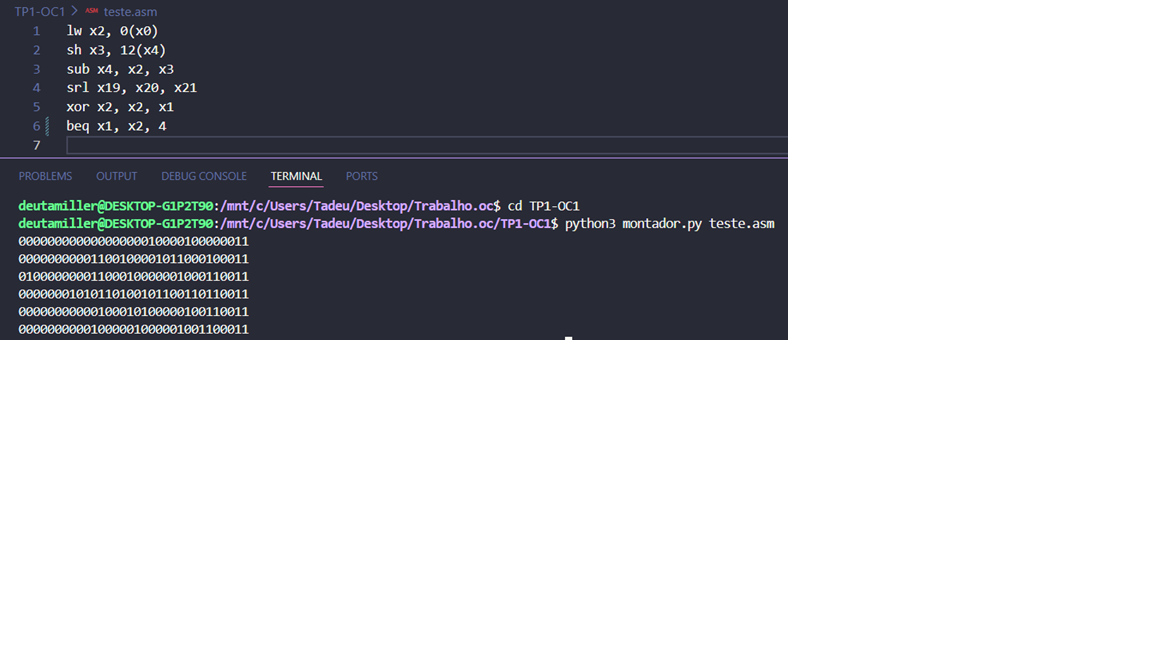
\includegraphics[width=0.8\textwidth]{teste.png}
\caption{Teste simulando um código com instruções mistas.}
\label{fig:teste_geral}
\end{figure}

\section{Conclusão}
A realização e construção do trabalho prático permitiu aprender de forma prática os conceitos vistos em sala de aula sobre as instruções da arquitetura RISC-V. Traduzir o assembly para binário deixou clara a importância de cada bit na formação do opcode, functs e registradores, além de mostrar como um montador funciona e conecta o software ao hardware.

O uso da linguagem Python se mostrou excelente, já que as funções nativas para lidar
com strings ajudaram na etapa de limpeza das linhas e separação dos argumentos, enquanto a lógica de dicionários tornou o processo de busca das instruções muito mais fácil do que uma estrutura cheia de ifs/elses. A principal complexidade durante o desenvolvimento foi a manipulação dos imediatos e o deslocamento de bits para o formato B, que exigiu um estudo de como a linguagem lida com representações binárias, complemento de dois em números negativos \cite{python_bitwise}.

Implementamos o reconhecimento de múltiplas bases numéricas (permitindo imediatos em binário ou hexadecimal, além do decimal) e suporte a pseudo instruções (como mv e li), conforme mencionado na seção de "Pontuação extra"na especificação do trabalho.

O link para o repositório do GitHub contendo o código do montador, casos de teste e README está disponível abaixo: https://github.com/arthurfcampos-png/oc-tp1

\bibliographystyle{sbc}
\bibliography{referencias}

\end{document}